\documentclass[11pt,a4paper]{article}
\usepackage[margin=2.2cm]{geometry}
\usepackage{amsmath,amssymb}
\usepackage{booktabs}
\usepackage{graphicx}
\usepackage{float}
\usepackage{pdflscape}
\usepackage[colorlinks=true,linkcolor=blue,urlcolor=blue]{hyperref}
\usepackage{caption}
\captionsetup{font=small}
\setlength{\parskip}{0.5em}
% Long \texttt{} identifiers (np.sqrt(samp).mean(axis=1), _metrics_frozen_rmse)
% cannot hyphenate and were overflowing the right margin; give TeX slack.
\setlength{\emergencystretch}{4em}
\sloppy
\title{\textbf{The Path-Shadowing RMSE Discrepancy}\\[0.3em]
\large Why the reproducibility report and the repository README disagree,\\
and what the number actually measures}
\author{\texttt{results/Heston/preprocessing\_with\_log\_returns}\\
BASSERAS/benchmark}
\date{31 July 2026}
\begin{document}
\maketitle

\tableofcontents
\clearpage

\section{The short answer}

Nothing was recomputed and no bank changed. \textbf{The two documents apply a
different final aggregation step to the same per-path errors}, and the CSDI
horizon-realised-volatility (rv) row is where the gap is widest.

\begin{center}
\begin{tabular}{llr}
\toprule
Source & Aggregation & CSDI rv RMSE @1M \\
\midrule
Report Table 8 (\S4.3, ``originally published'') & $\sqrt{\overline{se}}$ (root last) & 0.01772 \\
Report Table 5 (\S3.5, ``corrected'') & $\overline{\sqrt{se}}$ (root inside) & 0.01373 \\
Repository README (current) & $\overline{\sqrt{se}}$ (root inside) & 0.01373 \\
\bottomrule
\end{tabular}
\end{center}

So the discrepancy you spotted is \textbf{internal to the reproducibility
report}: it prints both conventions, in Table 8 and Table 5, without ever
showing them side by side. The README agrees with Table 5 to every printed
digit; it disagrees with Table 8 by a factor of 1.291. Only the RMSE rows differ
--- CRPS, coverage, width and miss-rate cells are identical between Table 8 and
Table 5, because those metrics are plain arithmetic means and are untouched by
the aggregation choice.


\section{How the RMSE is computed}

\subsection{From ensemble to per-path error}

Fix a held-out query path $q \in \{1,\dots,m\}$, $m = 512$, and a horizon step
$u \in \{1,\dots,H\}$. Path shadowing retrieves $K = 256$ nearest neighbours
from the bank and forms an ensemble forecast $Y_{q,u,k}$. The squared error of
the \emph{ensemble mean} against the realised value $y_{q,u}$ is
\[
se_{q,u} \;=\; \Bigl(\tfrac{1}{K}\textstyle\sum_{k=1}^{K} Y_{q,u,k} \;-\; y_{q,u}\Bigr)^{2},
\]
and each path is reduced to a single scalar by averaging over the horizon,
\[
se_q \;=\; \frac{1}{H}\sum_{u=1}^{H} se_{q,u}.
\]
Everything above is common to both documents. \textbf{The disagreement is
entirely in the last step}, which turns the length-$m$ vector $(se_q)$ into one
reported number.

\subsection{The two aggregations}

\[
\textbf{(A) root-last:}\quad R_A=\sqrt{\frac{1}{m}\sum_{q=1}^{m} se_q}
\qquad\qquad
\textbf{(B) root-inside:}\quad R_B=\frac{1}{m}\sum_{q=1}^{m}\sqrt{se_q}
\]

(A) is the textbook root-mean-square error: one square root, taken last. (B) is
the \emph{mean per-path root error} --- a square root per query path, then an
ordinary average.

Because $x \mapsto \sqrt{x}$ is \textbf{concave}, Jensen's inequality gives
\[
R_B \;=\; \mathbb{E}\bigl[\sqrt{se}\bigr] \;\le\; \sqrt{\mathbb{E}[se]} \;=\; R_A ,
\]
with equality if and only if every $se_q$ is identical. \textbf{(B) is therefore
always the smaller number}, and the gap widens as the spread of per-path errors
grows. This is why the effect is largest on rv: a scalar quantity with no
horizon averaging to smooth its error distribution.

\subsection{What the code actually does}

The shipped scorer (\texttt{path\_shadowing\_pdf.py}, \texttt{\_agg}) is
convention (B):

\begin{quote}\footnotesize\ttfamily
return float(np.sqrt(per).mean()) \\
\hspace*{2em} if kind == "rmse" else float(per.mean())
\end{quote}

\noindent
\texttt{np.sqrt(per).mean()} roots \emph{then} averages. The paired bootstrap
uses the matching form, \texttt{np.sqrt(samp).mean(axis=1)}, so the confidence
intervals are consistent with the point estimate.

\subsection{A naming caveat worth stating plainly}

Under convention (B) the reported quantity \textbf{is not a root-mean-square
error}, even though every table calls it ``RMSE''. For the scalar quantity rv
the horizon collapses ($H=1$), so $se_q = e_q^2$ and
\[
R_B=\frac{1}{m}\sum_q \sqrt{e_q^{2}}=\frac{1}{m}\sum_q |e_q| \;=\; \textbf{MAE exactly.}
\]
The rv ``RMSE'' row is a mean absolute error wearing the wrong label. For cum
and step it is a horizon-RMS averaged across paths --- a hybrid with no standard
name. This is inherited from the report, not invented here, but it should be
said out loud in any write-up that quotes the number.


\section{Why the difference exists}

The repository originally used (A). Commit \texttt{99977a3}, ``Align strict
path-shadowing RMSE with reproducibility report Table 5'', switched
\texttt{\_agg}, \texttt{\_boot\_ci} and the \texttt{terminal\_rmse} diagnostic
in all five scorers to (B) and re-ran the CSDI / LS4 / SBTS pipelines. Only the
RMSE fields moved; every other metric reproduced bit-identically, and the
Heston-oracle block stayed bit-identical across all three summaries.

The measured inflation $R_A/R_B$ at the 1M bank:

\begin{center}
\begin{tabular}{llrrr}
\toprule
Quantity & Method & (A) root-last & (B) root-inside & ratio $R_A/R_B$ \\
\midrule
cum & CSDI & 0.04925 & 0.04144 & 1.188 \\
cum & LS4 & 0.04894 & 0.04145 & 1.181 \\
cum & SBTS & 0.05523 & 0.04674 & 1.182 \\
step & CSDI & 0.01245 & 0.01176 & 1.059 \\
step & LS4 & 0.01245 & 0.01176 & 1.058 \\
step & SBTS & 0.01421 & 0.01350 & 1.053 \\
rv & CSDI & 0.01772 & 0.01373 & 1.291 \\
rv & LS4 & 0.01819 & 0.01426 & 1.276 \\
rv & SBTS & 0.01972 & 0.01541 & 1.279 \\
\bottomrule
\end{tabular}
\end{center}

The ratio is near-constant \emph{within} a quantity and very different
\emph{between} quantities ($\approx 1.18$ cum, $\approx 1.06$ step,
$\approx 1.28$ rv). That is the signature predicted above: the gap is set by the
dispersion of the per-path error distribution of the quantity, and across these
three \emph{generators} it barely moves.

One caveat, since it turned out to matter in \S5. That stability holds across
models of the \emph{same kind}; it is not a law. Re-running the two conditional
forecasters under (B) gave a cum ratio of $1.180$ and a step ratio of $1.056$,
both in line with the generators --- but an rv ratio of only $1.050$, against the
generators' $1.28$. Retrieval and direct forecasting produce differently
dispersed per-path rv errors, and the ratio follows the dispersion. So the ratio
may be used to \emph{anticipate} the size of a correction, never to substitute
for recomputing it.


\section{Three defects in the reproducibility report}

These are stated so the report can be corrected; none of them changes a number
in the tables of Section~\ref{sec:tables}.

\paragraph{1. \S2.7 describes the opposite of the shipped code.} The prose says
``the per-path squared errors are averaged over the evaluation set first, and a
\emph{single} square root is taken last'', and the accompanying listing prints
\texttt{np.sqrt(np.mean(per))} with the comment \texttt{\# per holds se\_i, NOT
sqrt(se\_i)}. The shipped code is \texttt{np.sqrt(per).mean()} --- the reverse.
The bootstrap listing is transposed in the same way. \S2.7 therefore documents
convention (A) while every table in the report except Table 8 is convention (B).

\paragraph{2. \S2.7 states Jensen's inequality backwards.} It claims the
mean-of-roots form ``is $\ge$ the above whenever the $se_i$ are not all equal,
and would overstate RMSE''. Since $\sqrt{\cdot}$ is concave the inequality runs
the other way: mean-of-roots \emph{under}states. The data confirms the direction
--- every ratio in the table above exceeds 1.

\paragraph{3. The Table 8 caption swaps the two labels.} It says Table 8's
column ``was produced with an earlier aggregation convention (mean of per-path
root errors)'' and that Table 5 ``follows the $\sqrt{\mathrm{mean}_i(se_i)}$
definition''. Both halves are inverted: Table 8 is the root-last form and
Table 5 is the mean-of-roots form. Table 8's numbers are uniformly \emph{larger},
which by Jensen is only possible if Table 8 is the root-last one. The caption on
Table 5 (``RMSE fixed to $\mathrm{mean}_i(\sqrt{se_i})$'') is the correct one,
and it contradicts both \S2.7 and the Table 8 caption.

\paragraph{Consequence.} The repository was aligned against a \emph{table
caption} that contradicts the report's own methods section. The alignment is
self-consistent and reproducible, but the report should be corrected so a reader
is not led to convention (A) by \S2.7.


\section{A mixed-convention defect in the tables --- found and fixed}

\textbf{Until 2026-07-31 the RMSE rows of the five tables below mixed both
conventions.} The four generators, the Heston oracle and the RW floor used (B).
The two conditional forecasters did not: \texttt{forecaster/pdf\_bridge.py}
pinned them to (A) through a local \texttt{\_metrics\_frozen\_rmse()}, so that a
re-run would reproduce the reproducibility report's published Chronos-2 /
TimesFM cells rather than silently drift away from them.

Because $R_B \le R_A$ always, this \textbf{systematically inflated the
forecasters' RMSE relative to every other column}. The defect was not cosmetic.
\texttt{build\_cross\_tables.py::\_ps\_winner\_idx} ranks \emph{all} model
columns, forecasters included, so the Winner column was silently comparing
inflated cells against un-inflated ones --- while the README footnote next to it
told the reader those cells were not comparable. A table cannot both rank a
number and disclaim it.

\textbf{The fix.} \texttt{\_metrics\_frozen\_rmse()} was deleted;
\texttt{score\_forecaster} now calls the shared \texttt{P.metrics\_with\_ci},
and the \texttt{terminal\_rmse} diagnostic was moved to
\texttt{np.abs(...).mean()} to match \texttt{eval\_bank} line 326 exactly. Both
forecasters were then re-run from their seed-0 recipes. Every non-RMSE leaf of
\texttt{chronos2\_pdf.json} and \texttt{timesfm\_pdf.json} reproduced
bit-identically (83 and 85 leaves respectively; CRPS, coverages, widths and miss
rates all unchanged to the last digit), which confirms the aggregation was the
only thing that moved.


\begin{center}\small
\begin{tabular}{llrrr}
\hline
Method & Quantity & before (A) & after (B) & ratio \\
\hline

Chronos-2 & cum & 0.04921 & 0.04168 & 1.180 \\

Chronos-2 & step & 0.01295 & 0.01227 & 1.056 \\

Chronos-2 & rv & 0.23075 & 0.21983 & 1.050 \\

TimesFM & cum & 0.05094 & 0.04276 & 1.191 \\

TimesFM & step & 0.01332 & 0.01267 & 1.051 \\

TimesFM & rv & 0.28650 & 0.25696 & 1.115 \\

\hline
\end{tabular}
\end{center}


\textbf{What it changes.} Chronos-2's cum RMSE falls from $0.04921$ to
$0.04168$, against CSDI's $0.04144$: a row that read as a $19\%$ deficit is a
$0.6\%$ one. The estimate offered before the re-run --- ``roughly $0.0416$'' from
the generator cum ratio --- was accurate for cum and step, but the rv ratio came
out at $1.050$ rather than the generators' $1.28$ (see the caveat in \S3), so
only the recomputation settles it.

\textbf{What it does not change.} Win counts were recomputed at all five bank
sizes and are identical: TimeDiT (raw) 14 at every bank, with CSDI 2 / SBTS 2 at
4\,096, CSDI 3 / SBTS 1 at 16\,384, and CSDI 3 / LS4 1 at the top three. CSDI
remains the row minimum for cum and step RMSE, so \textbf{no Winner cell moved}.
The tables in \S6 are the post-fix numbers.

\textbf{The cost.} The reproducibility report's published Chronos-2 / TimesFM
RMSE cells are now \emph{superseded, not reproduced} --- a re-run will no longer
match them, by design. That is the correct trade: one internally consistent
table is worth more than fidelity to a column the report itself never
recomputed. This is recorded in GUIDELINE E16b.

\clearpage
\section{The five cross-method tables}
\label{sec:tables}

Each table is one nested-prefix bank size of the \emph{same} 1M bank
(GUIDELINE \S9.1). Generator and oracle columns move with bank size; the
forecaster columns and the RW floor have no bank-size axis and repeat unchanged.
Winner excludes the oracle and RW floors. Width rows are diagnostics and carry
no winner: a degenerate zero-width interval would ``win'' while being completely
uncalibrated. \textbf{Bold} = best in row. TimeDiT's column is labelled
\textbf{TimeDiT (raw)} because its bank comes from the no-preprocessing
checkpoint; the protocol, $K=256$, query set, embedding, oracle and floor are
identical to the other generators.

\textbf{Every number below is generated by the same code path as the README
tables} (\texttt{build\_cross\_tables.py}), reading the same
\texttt{pdf\_summary.json} files, so the two cannot drift apart.

\begin{landscape}
\subsection{Bank size $N = 4\,096$}
\begin{center}\footnotesize
\begin{tabular}{lrrrrrrrrl}
\toprule
Quantity / metric & CSDI & TimeDiT (raw) & LS4 & SBTS & Chronos-2 & TimesFM & Oracle & RW & Winner \\
\midrule
\multicolumn{10}{l}{\textbf{cum ($M\times H$ trajectory)}} \\
RMSE $\downarrow$ & \textbf{0.04131} & 0.04142 & 0.04149 & 0.04158 & 0.04168 & 0.04276 & 0.04154 & 0.04796 & \textbf{CSDI} \\
CRPS $\downarrow$ & 0.02548 & \textbf{0.02531} & 0.02544 & 0.02544 & 0.02624 & 0.02722 & 0.02539 & 0.02946 & \textbf{TimeDiT (raw)} \\
coverage$_{50}$ ($\to$0.50) & 0.4571 & \textbf{0.5105} & 0.4764 & 0.4839 & 0.4050 & 0.4664 & 0.4875 & 0.4719 & \textbf{TimeDiT (raw)} \\
coverage$_{90}$ ($\to$0.90) & 0.8629 & \textbf{0.8957} & 0.8691 & 0.8805 & 0.7905 & 0.8177 & 0.8919 & 0.8553 & \textbf{TimeDiT (raw)} \\
width$_{50}$ (diag) & 0.05070 & 0.05901 & 0.05376 & 0.05536 & 0.04454 & 0.05477 & 0.05573 & 0.06286 & --- \\
width$_{90}$ (diag) & 0.1318 & 0.1488 & 0.1353 & 0.1439 & 0.1166 & 0.1348 & 0.1462 & 0.1520 & --- \\
lower miss$_{90}$ ($\to$0.05) & 0.07764 & \textbf{0.04840} & 0.06476 & 0.05554 & 0.09595 & 0.09265 & 0.05731 & 0.08331 & \textbf{TimeDiT (raw)} \\
upper miss$_{90}$ ($\to$0.05) & 0.05945 & \textbf{0.05591} & 0.06616 & 0.06396 & 0.1135 & 0.08966 & 0.05078 & 0.06134 & \textbf{TimeDiT (raw)} \\
\addlinespace
\multicolumn{10}{l}{\textbf{step ($M\times H$)}} \\
RMSE $\downarrow$ & \textbf{0.01176} & 0.01177 & 0.01176 & 0.01180 & 0.01227 & 0.01267 & 0.01176 & 0.01185 & \textbf{CSDI} \\
CRPS $\downarrow$ & 0.006780 & \textbf{0.006766} & 0.006794 & 0.006812 & 0.01272 & 0.01473 & 0.006765 & 0.006874 & \textbf{TimeDiT (raw)} \\
coverage$_{50}$ ($\to$0.50) & 0.4510 & 0.4811 & 0.4656 & \textbf{0.4813} & 0.9449 & 0.9479 & 0.4849 & 0.5157 & \textbf{SBTS} \\
coverage$_{90}$ ($\to$0.90) & 0.8602 & \textbf{0.8854} & 0.8591 & 0.8782 & 0.9970 & 0.9949 & 0.8869 & 0.8866 & \textbf{TimeDiT (raw)} \\
width$_{50}$ (diag) & 0.01321 & 0.01429 & 0.01359 & 0.01434 & 0.06405 & 0.07667 & 0.01434 & 0.01602 & --- \\
width$_{90}$ (diag) & 0.03524 & 0.03794 & 0.03530 & 0.03769 & 0.1609 & 0.1801 & 0.03828 & 0.03968 & --- \\
lower miss$_{90}$ ($\to$0.05) & 0.07098 & \textbf{0.05573} & 0.07233 & 0.05890 & 0.001770 & 0.002319 & 0.05676 & 0.05933 & \textbf{TimeDiT (raw)} \\
upper miss$_{90}$ ($\to$0.05) & 0.06885 & \textbf{0.05884} & 0.06860 & 0.06287 & 0.001221 & 0.002808 & 0.05634 & 0.05408 & \textbf{TimeDiT (raw)} \\
\addlinespace
\multicolumn{10}{l}{\textbf{rv ($M$ scalar)}} \\
RMSE $\downarrow$ & 0.01458 & \textbf{0.01364} & 0.01516 & 0.01420 & 0.2198 & 0.2570 & 0.01381 & 0.01509 & \textbf{TimeDiT (raw)} \\
CRPS $\downarrow$ & 0.01055 & \textbf{0.009653} & 0.01098 & 0.01010 & 0.1913 & 0.2291 & 0.009777 & 0.01168 & \textbf{TimeDiT (raw)} \\
coverage$_{50}$ ($\to$0.50) & 0.4609 & \textbf{0.4805} & 0.4121 & 0.4805 & 0 & 0 & 0.5059 & 0.2344 & \textbf{TimeDiT (raw)} \\
coverage$_{90}$ ($\to$0.90) & 0.8594 & \textbf{0.8945} & 0.7812 & 0.8652 & 0 & 0.001953 & 0.9141 & 0.5332 & \textbf{TimeDiT (raw)} \\
width$_{50}$ (diag) & 0.02220 & 0.02273 & 0.02027 & 0.02287 & 0.06861 & 0.06689 & 0.02404 & 0.01202 & --- \\
width$_{90}$ (diag) & 0.05413 & 0.05489 & 0.04837 & 0.05458 & 0.1651 & 0.1610 & 0.05753 & 0.02873 & --- \\
lower miss$_{90}$ ($\to$0.05) & 0.01758 & 0.04102 & 0.05664 & \textbf{0.05078} & 1.000 & 0.9980 & 0.02734 & 0.2891 & \textbf{SBTS} \\
upper miss$_{90}$ ($\to$0.05) & 0.1230 & \textbf{0.06445} & 0.1621 & 0.08398 & 0 & 0 & 0.05859 & 0.1777 & \textbf{TimeDiT (raw)} \\
\bottomrule
\end{tabular}
\end{center}
\noindent\textbf{Winners (of 18 ranked rows = 6 ranked metrics $\times$ 3 quantities):} TimeDiT (raw) 14 $\cdot$ CSDI 2 $\cdot$ SBTS 2.
\end{landscape}
\begin{landscape}
\subsection{Bank size $N = 16\,384$}
\begin{center}\footnotesize
\begin{tabular}{lrrrrrrrrl}
\toprule
Quantity / metric & CSDI & TimeDiT (raw) & LS4 & SBTS & Chronos-2 & TimesFM & Oracle & RW & Winner \\
\midrule
\multicolumn{10}{l}{\textbf{cum ($M\times H$ trajectory)}} \\
RMSE $\downarrow$ & \textbf{0.04142} & 0.04156 & 0.04150 & 0.04234 & 0.04168 & 0.04276 & 0.04155 & 0.04796 & \textbf{CSDI} \\
CRPS $\downarrow$ & 0.02543 & \textbf{0.02534} & 0.02542 & 0.02610 & 0.02624 & 0.02722 & 0.02535 & 0.02946 & \textbf{TimeDiT (raw)} \\
coverage$_{50}$ ($\to$0.50) & 0.4604 & \textbf{0.5103} & 0.4755 & 0.4694 & 0.4050 & 0.4664 & 0.4859 & 0.4719 & \textbf{TimeDiT (raw)} \\
coverage$_{90}$ ($\to$0.90) & 0.8694 & \textbf{0.8952} & 0.8685 & 0.8644 & 0.7905 & 0.8177 & 0.8884 & 0.8553 & \textbf{TimeDiT (raw)} \\
width$_{50}$ (diag) & 0.05197 & 0.05936 & 0.05375 & 0.05538 & 0.04454 & 0.05477 & 0.05606 & 0.06286 & --- \\
width$_{90}$ (diag) & 0.1348 & 0.1484 & 0.1357 & 0.1410 & 0.1166 & 0.1348 & 0.1446 & 0.1520 & --- \\
lower miss$_{90}$ ($\to$0.05) & 0.07318 & \textbf{0.04651} & 0.06458 & 0.06787 & 0.09595 & 0.09265 & 0.05731 & 0.08331 & \textbf{TimeDiT (raw)} \\
upper miss$_{90}$ ($\to$0.05) & \textbf{0.05743} & 0.05829 & 0.06689 & 0.06769 & 0.1135 & 0.08966 & 0.05432 & 0.06134 & \textbf{CSDI} \\
\addlinespace
\multicolumn{10}{l}{\textbf{step ($M\times H$)}} \\
RMSE $\downarrow$ & \textbf{0.01176} & 0.01177 & 0.01176 & 0.01192 & 0.01227 & 0.01267 & 0.01176 & 0.01185 & \textbf{CSDI} \\
CRPS $\downarrow$ & 0.006777 & \textbf{0.006768} & 0.006788 & 0.006930 & 0.01272 & 0.01473 & 0.006761 & 0.006874 & \textbf{TimeDiT (raw)} \\
coverage$_{50}$ ($\to$0.50) & 0.4493 & \textbf{0.4818} & 0.4648 & 0.4751 & 0.9449 & 0.9479 & 0.4810 & 0.5157 & \textbf{TimeDiT (raw)} \\
coverage$_{90}$ ($\to$0.90) & 0.8639 & \textbf{0.8843} & 0.8630 & 0.8624 & 0.9970 & 0.9949 & 0.8862 & 0.8866 & \textbf{TimeDiT (raw)} \\
width$_{50}$ (diag) & 0.01326 & 0.01431 & 0.01365 & 0.01444 & 0.06405 & 0.07667 & 0.01437 & 0.01602 & --- \\
width$_{90}$ (diag) & 0.03534 & 0.03781 & 0.03544 & 0.03709 & 0.1609 & 0.1801 & 0.03807 & 0.03968 & --- \\
lower miss$_{90}$ ($\to$0.05) & 0.07104 & \textbf{0.05719} & 0.06995 & 0.06750 & 0.001770 & 0.002319 & 0.05762 & 0.05933 & \textbf{TimeDiT (raw)} \\
upper miss$_{90}$ ($\to$0.05) & 0.06506 & \textbf{0.05847} & 0.06702 & 0.07013 & 0.001221 & 0.002808 & 0.05621 & 0.05408 & \textbf{TimeDiT (raw)} \\
\addlinespace
\multicolumn{10}{l}{\textbf{rv ($M$ scalar)}} \\
RMSE $\downarrow$ & 0.01421 & \textbf{0.01341} & 0.01470 & 0.01414 & 0.2198 & 0.2570 & 0.01347 & 0.01509 & \textbf{TimeDiT (raw)} \\
CRPS $\downarrow$ & 0.01028 & \textbf{0.009484} & 0.01066 & 0.01009 & 0.1913 & 0.2291 & 0.009513 & 0.01168 & \textbf{TimeDiT (raw)} \\
coverage$_{50}$ ($\to$0.50) & 0.4570 & \textbf{0.4883} & 0.4199 & 0.4629 & 0 & 0 & 0.4961 & 0.2344 & \textbf{TimeDiT (raw)} \\
coverage$_{90}$ ($\to$0.90) & 0.8691 & \textbf{0.8926} & 0.7871 & 0.8574 & 0 & 0.001953 & 0.9141 & 0.5332 & \textbf{TimeDiT (raw)} \\
width$_{50}$ (diag) & 0.02189 & 0.02217 & 0.01990 & 0.02194 & 0.06861 & 0.06689 & 0.02286 & 0.01202 & --- \\
width$_{90}$ (diag) & 0.05318 & 0.05322 & 0.04786 & 0.05252 & 0.1651 & 0.1610 & 0.05559 & 0.02873 & --- \\
lower miss$_{90}$ ($\to$0.05) & 0.01562 & 0.03906 & 0.05469 & \textbf{0.05273} & 1.000 & 0.9980 & 0.03125 & 0.2891 & \textbf{SBTS} \\
upper miss$_{90}$ ($\to$0.05) & 0.1152 & \textbf{0.06836} & 0.1582 & 0.08984 & 0 & 0 & 0.05469 & 0.1777 & \textbf{TimeDiT (raw)} \\
\bottomrule
\end{tabular}
\end{center}
\noindent\textbf{Winners (of 18 ranked rows = 6 ranked metrics $\times$ 3 quantities):} TimeDiT (raw) 14 $\cdot$ CSDI 3 $\cdot$ SBTS 1.
\end{landscape}
\begin{landscape}
\subsection{Bank size $N = 65\,536$}
\begin{center}\footnotesize
\begin{tabular}{lrrrrrrrrl}
\toprule
Quantity / metric & CSDI & TimeDiT (raw) & LS4 & SBTS & Chronos-2 & TimesFM & Oracle & RW & Winner \\
\midrule
\multicolumn{10}{l}{\textbf{cum ($M\times H$ trajectory)}} \\
RMSE $\downarrow$ & \textbf{0.04130} & 0.04161 & 0.04148 & 0.04389 & 0.04168 & 0.04276 & 0.04140 & 0.04796 & \textbf{CSDI} \\
CRPS $\downarrow$ & 0.02535 & \textbf{0.02533} & 0.02536 & 0.02768 & 0.02624 & 0.02722 & 0.02524 & 0.02946 & \textbf{TimeDiT (raw)} \\
coverage$_{50}$ ($\to$0.50) & 0.4670 & \textbf{0.5046} & 0.4717 & 0.4256 & 0.4050 & 0.4664 & 0.4886 & 0.4719 & \textbf{TimeDiT (raw)} \\
coverage$_{90}$ ($\to$0.90) & 0.8738 & \textbf{0.8970} & 0.8685 & 0.8198 & 0.7905 & 0.8177 & 0.8887 & 0.8553 & \textbf{TimeDiT (raw)} \\
width$_{50}$ (diag) & 0.05283 & 0.05886 & 0.05369 & 0.05231 & 0.04454 & 0.05477 & 0.05630 & 0.06286 & --- \\
width$_{90}$ (diag) & 0.1354 & 0.1480 & 0.1353 & 0.1309 & 0.1166 & 0.1348 & 0.1448 & 0.1520 & --- \\
lower miss$_{90}$ ($\to$0.05) & 0.07147 & \textbf{0.04761} & 0.06500 & 0.08795 & 0.09595 & 0.09265 & 0.05688 & 0.08331 & \textbf{TimeDiT (raw)} \\
upper miss$_{90}$ ($\to$0.05) & \textbf{0.05469} & 0.05536 & 0.06647 & 0.09229 & 0.1135 & 0.08966 & 0.05444 & 0.06134 & \textbf{CSDI} \\
\addlinespace
\multicolumn{10}{l}{\textbf{step ($M\times H$)}} \\
RMSE $\downarrow$ & \textbf{0.01175} & 0.01177 & 0.01177 & 0.01228 & 0.01227 & 0.01267 & 0.01176 & 0.01185 & \textbf{CSDI} \\
CRPS $\downarrow$ & 0.006770 & \textbf{0.006762} & 0.006786 & 0.007304 & 0.01272 & 0.01473 & 0.006754 & 0.006874 & \textbf{TimeDiT (raw)} \\
coverage$_{50}$ ($\to$0.50) & 0.4486 & \textbf{0.4765} & 0.4667 & 0.4406 & 0.9449 & 0.9479 & 0.4820 & 0.5157 & \textbf{TimeDiT (raw)} \\
coverage$_{90}$ ($\to$0.90) & 0.8639 & \textbf{0.8810} & 0.8627 & 0.8183 & 0.9970 & 0.9949 & 0.8864 & 0.8866 & \textbf{TimeDiT (raw)} \\
width$_{50}$ (diag) & 0.01330 & 0.01423 & 0.01367 & 0.01400 & 0.06405 & 0.07667 & 0.01441 & 0.01602 & --- \\
width$_{90}$ (diag) & 0.03542 & 0.03760 & 0.03538 & 0.03433 & 0.1609 & 0.1801 & 0.03807 & 0.03968 & --- \\
lower miss$_{90}$ ($\to$0.05) & 0.07001 & \textbf{0.05884} & 0.07025 & 0.08905 & 0.001770 & 0.002319 & 0.05658 & 0.05933 & \textbf{TimeDiT (raw)} \\
upper miss$_{90}$ ($\to$0.05) & 0.06610 & \textbf{0.06012} & 0.06708 & 0.09265 & 0.001221 & 0.002808 & 0.05701 & 0.05408 & \textbf{TimeDiT (raw)} \\
\addlinespace
\multicolumn{10}{l}{\textbf{rv ($M$ scalar)}} \\
RMSE $\downarrow$ & 0.01393 & \textbf{0.01327} & 0.01448 & 0.01432 & 0.2198 & 0.2570 & 0.01314 & 0.01509 & \textbf{TimeDiT (raw)} \\
CRPS $\downarrow$ & 0.01007 & \textbf{0.009409} & 0.01048 & 0.01058 & 0.1913 & 0.2291 & 0.009330 & 0.01168 & \textbf{TimeDiT (raw)} \\
coverage$_{50}$ ($\to$0.50) & 0.4551 & \textbf{0.4902} & 0.4141 & 0.4258 & 0 & 0 & 0.4980 & 0.2344 & \textbf{TimeDiT (raw)} \\
coverage$_{90}$ ($\to$0.90) & 0.8652 & \textbf{0.8945} & 0.7910 & 0.8262 & 0 & 0.001953 & 0.9199 & 0.5332 & \textbf{TimeDiT (raw)} \\
width$_{50}$ (diag) & 0.02148 & 0.02197 & 0.01961 & 0.02067 & 0.06861 & 0.06689 & 0.02259 & 0.01202 & --- \\
width$_{90}$ (diag) & 0.05219 & 0.05302 & 0.04666 & 0.04806 & 0.1651 & 0.1610 & 0.05502 & 0.02873 & --- \\
lower miss$_{90}$ ($\to$0.05) & 0.01562 & 0.03711 & \textbf{0.05078} & 0.06445 & 1.000 & 0.9980 & 0.02930 & 0.2891 & \textbf{LS4} \\
upper miss$_{90}$ ($\to$0.05) & 0.1191 & \textbf{0.06836} & 0.1582 & 0.1094 & 0 & 0 & 0.05078 & 0.1777 & \textbf{TimeDiT (raw)} \\
\bottomrule
\end{tabular}
\end{center}
\noindent\textbf{Winners (of 18 ranked rows = 6 ranked metrics $\times$ 3 quantities):} TimeDiT (raw) 14 $\cdot$ CSDI 3 $\cdot$ LS4 1.
\end{landscape}
\begin{landscape}
\subsection{Bank size $N = 262\,144$}
\begin{center}\footnotesize
\begin{tabular}{lrrrrrrrrl}
\toprule
Quantity / metric & CSDI & TimeDiT (raw) & LS4 & SBTS & Chronos-2 & TimesFM & Oracle & RW & Winner \\
\midrule
\multicolumn{10}{l}{\textbf{cum ($M\times H$ trajectory)}} \\
RMSE $\downarrow$ & \textbf{0.04138} & 0.04152 & 0.04149 & 0.04540 & 0.04168 & 0.04276 & 0.04136 & 0.04796 & \textbf{CSDI} \\
CRPS $\downarrow$ & 0.02541 & \textbf{0.02528} & 0.02536 & 0.02987 & 0.02624 & 0.02722 & 0.02524 & 0.02946 & \textbf{TimeDiT (raw)} \\
coverage$_{50}$ ($\to$0.50) & 0.4644 & \textbf{0.5010} & 0.4723 & 0.3552 & 0.4050 & 0.4664 & 0.4904 & 0.4719 & \textbf{TimeDiT (raw)} \\
coverage$_{90}$ ($\to$0.90) & 0.8691 & \textbf{0.8972} & 0.8696 & 0.7396 & 0.7905 & 0.8177 & 0.8922 & 0.8553 & \textbf{TimeDiT (raw)} \\
width$_{50}$ (diag) & 0.05267 & 0.05879 & 0.05349 & 0.04573 & 0.04454 & 0.05477 & 0.05706 & 0.06286 & --- \\
width$_{90}$ (diag) & 0.1344 & 0.1480 & 0.1350 & 0.1137 & 0.1166 & 0.1348 & 0.1460 & 0.1520 & --- \\
lower miss$_{90}$ ($\to$0.05) & 0.07501 & \textbf{0.04675} & 0.06653 & 0.1324 & 0.09595 & 0.09265 & 0.05548 & 0.08331 & \textbf{TimeDiT (raw)} \\
upper miss$_{90}$ ($\to$0.05) & \textbf{0.05591} & 0.05609 & 0.06384 & 0.1280 & 0.1135 & 0.08966 & 0.05231 & 0.06134 & \textbf{CSDI} \\
\addlinespace
\multicolumn{10}{l}{\textbf{step ($M\times H$)}} \\
RMSE $\downarrow$ & \textbf{0.01176} & 0.01177 & 0.01177 & 0.01290 & 0.01227 & 0.01267 & 0.01176 & 0.01185 & \textbf{CSDI} \\
CRPS $\downarrow$ & 0.006771 & \textbf{0.006760} & 0.006784 & 0.008009 & 0.01272 & 0.01473 & 0.006752 & 0.006874 & \textbf{TimeDiT (raw)} \\
coverage$_{50}$ ($\to$0.50) & 0.4529 & \textbf{0.4753} & 0.4653 & 0.3699 & 0.9449 & 0.9479 & 0.4825 & 0.5157 & \textbf{TimeDiT (raw)} \\
coverage$_{90}$ ($\to$0.90) & 0.8638 & \textbf{0.8822} & 0.8645 & 0.7321 & 0.9970 & 0.9949 & 0.8849 & 0.8866 & \textbf{TimeDiT (raw)} \\
width$_{50}$ (diag) & 0.01332 & 0.01425 & 0.01367 & 0.01230 & 0.06405 & 0.07667 & 0.01444 & 0.01602 & --- \\
width$_{90}$ (diag) & 0.03547 & 0.03759 & 0.03538 & 0.02975 & 0.1609 & 0.1801 & 0.03806 & 0.03968 & --- \\
lower miss$_{90}$ ($\to$0.05) & 0.07080 & \textbf{0.05811} & 0.06830 & 0.1332 & 0.001770 & 0.002319 & 0.05829 & 0.05933 & \textbf{TimeDiT (raw)} \\
upper miss$_{90}$ ($\to$0.05) & 0.06543 & \textbf{0.05969} & 0.06720 & 0.1347 & 0.001221 & 0.002808 & 0.05682 & 0.05408 & \textbf{TimeDiT (raw)} \\
\addlinespace
\multicolumn{10}{l}{\textbf{rv ($M$ scalar)}} \\
RMSE $\downarrow$ & 0.01379 & \textbf{0.01305} & 0.01433 & 0.01487 & 0.2198 & 0.2570 & 0.01306 & 0.01509 & \textbf{TimeDiT (raw)} \\
CRPS $\downarrow$ & 0.009987 & \textbf{0.009273} & 0.01038 & 0.01155 & 0.1913 & 0.2291 & 0.009256 & 0.01168 & \textbf{TimeDiT (raw)} \\
coverage$_{50}$ ($\to$0.50) & 0.4609 & \textbf{0.4902} & 0.4277 & 0.3496 & 0 & 0 & 0.4922 & 0.2344 & \textbf{TimeDiT (raw)} \\
coverage$_{90}$ ($\to$0.90) & 0.8672 & \textbf{0.8926} & 0.8105 & 0.7500 & 0 & 0.001953 & 0.9180 & 0.5332 & \textbf{TimeDiT (raw)} \\
width$_{50}$ (diag) & 0.02140 & 0.02177 & 0.01929 & 0.01770 & 0.06861 & 0.06689 & 0.02231 & 0.01202 & --- \\
width$_{90}$ (diag) & 0.05196 & 0.05261 & 0.04621 & 0.04149 & 0.1651 & 0.1610 & 0.05430 & 0.02873 & --- \\
lower miss$_{90}$ ($\to$0.05) & 0.01758 & 0.03906 & \textbf{0.04688} & 0.09766 & 1.000 & 0.9980 & 0.03125 & 0.2891 & \textbf{LS4} \\
upper miss$_{90}$ ($\to$0.05) & 0.1152 & \textbf{0.06836} & 0.1426 & 0.1523 & 0 & 0 & 0.05078 & 0.1777 & \textbf{TimeDiT (raw)} \\
\bottomrule
\end{tabular}
\end{center}
\noindent\textbf{Winners (of 18 ranked rows = 6 ranked metrics $\times$ 3 quantities):} TimeDiT (raw) 14 $\cdot$ CSDI 3 $\cdot$ LS4 1.
\end{landscape}
\begin{landscape}
\subsection{Bank size $N = 1\,000\,000$}
\begin{center}\footnotesize
\begin{tabular}{lrrrrrrrrl}
\toprule
Quantity / metric & CSDI & TimeDiT (raw) & LS4 & SBTS & Chronos-2 & TimesFM & Oracle & RW & Winner \\
\midrule
\multicolumn{10}{l}{\textbf{cum ($M\times H$ trajectory)}} \\
RMSE $\downarrow$ & \textbf{0.04144} & 0.04145 & 0.04145 & 0.04674 & 0.04168 & 0.04276 & 0.04148 & 0.04796 & \textbf{CSDI} \\
CRPS $\downarrow$ & 0.02544 & \textbf{0.02521} & 0.02534 & 0.03179 & 0.02624 & 0.02722 & 0.02525 & 0.02946 & \textbf{TimeDiT (raw)} \\
coverage$_{50}$ ($\to$0.50) & 0.4624 & \textbf{0.5072} & 0.4688 & 0.3001 & 0.4050 & 0.4664 & 0.4891 & 0.4719 & \textbf{TimeDiT (raw)} \\
coverage$_{90}$ ($\to$0.90) & 0.8682 & \textbf{0.8983} & 0.8682 & 0.6575 & 0.7905 & 0.8177 & 0.8941 & 0.8553 & \textbf{TimeDiT (raw)} \\
width$_{50}$ (diag) & 0.05285 & 0.05901 & 0.05359 & 0.04003 & 0.04454 & 0.05477 & 0.05719 & 0.06286 & --- \\
width$_{90}$ (diag) & 0.1348 & 0.1486 & 0.1349 & 0.09761 & 0.1166 & 0.1348 & 0.1465 & 0.1520 & --- \\
lower miss$_{90}$ ($\to$0.05) & 0.07599 & \textbf{0.04572} & 0.06757 & 0.1738 & 0.09595 & 0.09265 & 0.05463 & 0.08331 & \textbf{TimeDiT (raw)} \\
upper miss$_{90}$ ($\to$0.05) & \textbf{0.05579} & 0.05597 & 0.06427 & 0.1687 & 0.1135 & 0.08966 & 0.05127 & 0.06134 & \textbf{CSDI} \\
\addlinespace
\multicolumn{10}{l}{\textbf{step ($M\times H$)}} \\
RMSE $\downarrow$ & \textbf{0.01176} & 0.01178 & 0.01176 & 0.01350 & 0.01227 & 0.01267 & 0.01176 & 0.01185 & \textbf{CSDI} \\
CRPS $\downarrow$ & 0.006767 & \textbf{0.006760} & 0.006778 & 0.008688 & 0.01272 & 0.01473 & 0.006750 & 0.006874 & \textbf{TimeDiT (raw)} \\
coverage$_{50}$ ($\to$0.50) & 0.4532 & \textbf{0.4761} & 0.4672 & 0.3082 & 0.9449 & 0.9479 & 0.4816 & 0.5157 & \textbf{TimeDiT (raw)} \\
coverage$_{90}$ ($\to$0.90) & 0.8640 & \textbf{0.8806} & 0.8640 & 0.6479 & 0.9970 & 0.9949 & 0.8864 & 0.8866 & \textbf{TimeDiT (raw)} \\
width$_{50}$ (diag) & 0.01338 & 0.01428 & 0.01368 & 0.01071 & 0.06405 & 0.07667 & 0.01449 & 0.01602 & --- \\
width$_{90}$ (diag) & 0.03550 & 0.03758 & 0.03538 & 0.02568 & 0.1609 & 0.1801 & 0.03815 & 0.03968 & --- \\
lower miss$_{90}$ ($\to$0.05) & 0.07062 & \textbf{0.05884} & 0.06921 & 0.1762 & 0.001770 & 0.002319 & 0.05725 & 0.05933 & \textbf{TimeDiT (raw)} \\
upper miss$_{90}$ ($\to$0.05) & 0.06543 & \textbf{0.06061} & 0.06683 & 0.1758 & 0.001221 & 0.002808 & 0.05634 & 0.05408 & \textbf{TimeDiT (raw)} \\
\addlinespace
\multicolumn{10}{l}{\textbf{rv ($M$ scalar)}} \\
RMSE $\downarrow$ & 0.01373 & \textbf{0.01295} & 0.01426 & 0.01541 & 0.2198 & 0.2570 & 0.01291 & 0.01509 & \textbf{TimeDiT (raw)} \\
CRPS $\downarrow$ & 0.009938 & \textbf{0.009179} & 0.01032 & 0.01241 & 0.1913 & 0.2291 & 0.009143 & 0.01168 & \textbf{TimeDiT (raw)} \\
coverage$_{50}$ ($\to$0.50) & 0.4746 & \textbf{0.4883} & 0.4102 & 0.2930 & 0 & 0 & 0.4727 & 0.2344 & \textbf{TimeDiT (raw)} \\
coverage$_{90}$ ($\to$0.90) & 0.8633 & \textbf{0.8945} & 0.7988 & 0.6641 & 0 & 0.001953 & 0.9238 & 0.5332 & \textbf{TimeDiT (raw)} \\
width$_{50}$ (diag) & 0.02115 & 0.02155 & 0.01914 & 0.01493 & 0.06861 & 0.06689 & 0.02217 & 0.01202 & --- \\
width$_{90}$ (diag) & 0.05138 & 0.05213 & 0.04589 & 0.03608 & 0.1651 & 0.1610 & 0.05411 & 0.02873 & --- \\
lower miss$_{90}$ ($\to$0.05) & 0.01758 & 0.03125 & \textbf{0.05078} & 0.1328 & 1.000 & 0.9980 & 0.02930 & 0.2891 & \textbf{LS4} \\
upper miss$_{90}$ ($\to$0.05) & 0.1191 & \textbf{0.07422} & 0.1504 & 0.2031 & 0 & 0 & 0.04688 & 0.1777 & \textbf{TimeDiT (raw)} \\
\bottomrule
\end{tabular}
\end{center}
\noindent\textbf{Winners (of 18 ranked rows = 6 ranked metrics $\times$ 3 quantities):} TimeDiT (raw) 14 $\cdot$ CSDI 3 $\cdot$ LS4 1.
\end{landscape}
\clearpage
\section{Figures}

Every figure in the experiment folder, grouped. The eight-panel diagnostics are,
row by row: real vs generated path bundles; log-return density and QQ vs real;
ACF of $|r|$ and ACF of $r^2$; 5-day rolling-volatility density and
terminal-price tail survival (log-log). Blue = real test set, red/orange =
generated, dashed = theoretical or empirical reference.

\textbf{Known caption artefact:} the path-bundle panel titles read ``8192
total''; the true count is 4096. The shared plotter
\texttt{metrics/plot\_diagnostics.py} hardcodes 8192 (lines 151/160) from the
main benchmark. The plotted data is the correct 4096-path test set --- only the
string is stale, it affects all four methods identically, and it changes no
number in any table.

\subsection{Stylised-fact diagnostics (8-panel)}
\begin{figure}[H]
\centering

\includegraphics[width=\linewidth]{../CSDI/plots/heston_diagnostics.png}
\caption{CSDI --- log-return preprocessing. Eight-panel Heston stylised-fact diagnostics (seed 0).}
\end{figure}
\begin{figure}[H]
\centering

\includegraphics[width=\linewidth]{../CSDI/baseline_no_preproc/plots/heston_diagnostics.png}
\caption{CSDI --- raw price, no preprocessing. Eight-panel Heston stylised-fact diagnostics (seed 0).}
\end{figure}
\begin{figure}[H]
\centering

\includegraphics[width=\linewidth]{../TimeDiT/plots/heston_diagnostics.png}
\caption{TimeDiT --- log-return preprocessing. Eight-panel Heston stylised-fact diagnostics (seed 0).}
\end{figure}
\begin{figure}[H]
\centering

\includegraphics[width=\linewidth]{../TimeDiT/baseline_no_preproc/plots/heston_diagnostics.png}
\caption{TimeDiT --- raw price, no preprocessing. Eight-panel Heston stylised-fact diagnostics (seed 0).}
\end{figure}
\begin{figure}[H]
\centering

\includegraphics[width=\linewidth]{../LS4/plots/heston_diagnostics.png}
\caption{LS4 --- log-return preprocessing. Eight-panel Heston stylised-fact diagnostics (seed 0).}
\end{figure}
\begin{figure}[H]
\centering

\includegraphics[width=\linewidth]{../LS4/baseline_no_preproc/plots/heston_diagnostics.png}
\caption{LS4 --- raw price, no preprocessing. Eight-panel Heston stylised-fact diagnostics (seed 0).}
\end{figure}
\begin{figure}[H]
\centering

\includegraphics[width=\linewidth]{../SBTS/plots/heston_diagnostics.png}
\caption{SBTS --- log-return preprocessing. Eight-panel Heston stylised-fact diagnostics (seed 0).}
\end{figure}
\begin{figure}[H]
\centering

\includegraphics[width=\linewidth]{../SBTS/baseline_no_preproc/plots/heston_diagnostics.png}
\caption{SBTS --- raw price, no preprocessing. Eight-panel Heston stylised-fact diagnostics (seed 0).}
\end{figure}
\subsection{Path-shadowing convergence and calibration}
\begin{figure}[H]
\centering
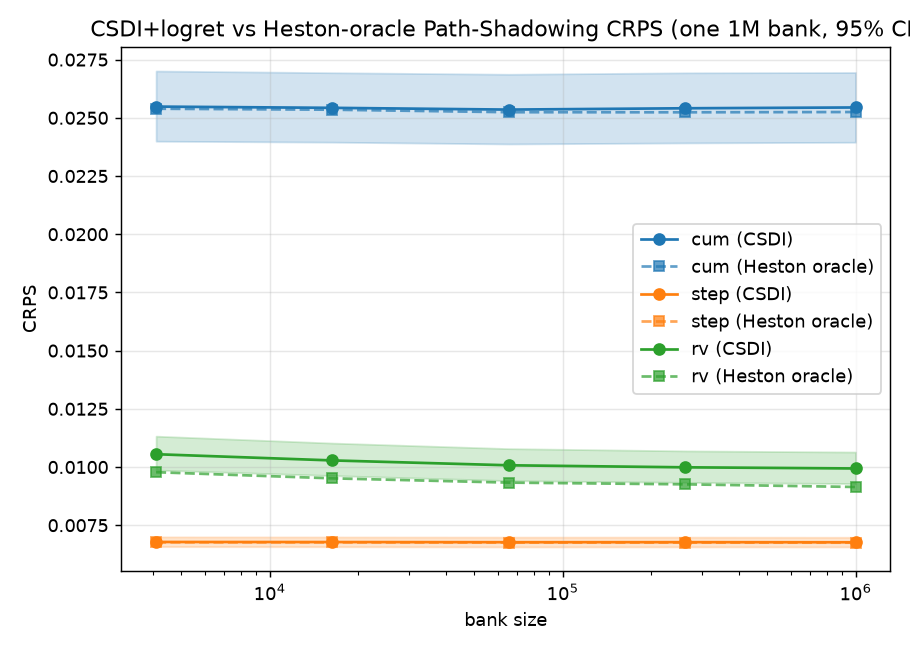
\includegraphics[width=\linewidth]{../CSDI/path_shadowing/plots/pdf_crps_vs_banksize.png}
\caption{CSDI --- CRPS vs bank size (log $x$); solid = generator, dashed = size-matched Heston oracle, shaded = 95\% bootstrap band.}
\end{figure}
\begin{figure}[H]
\centering
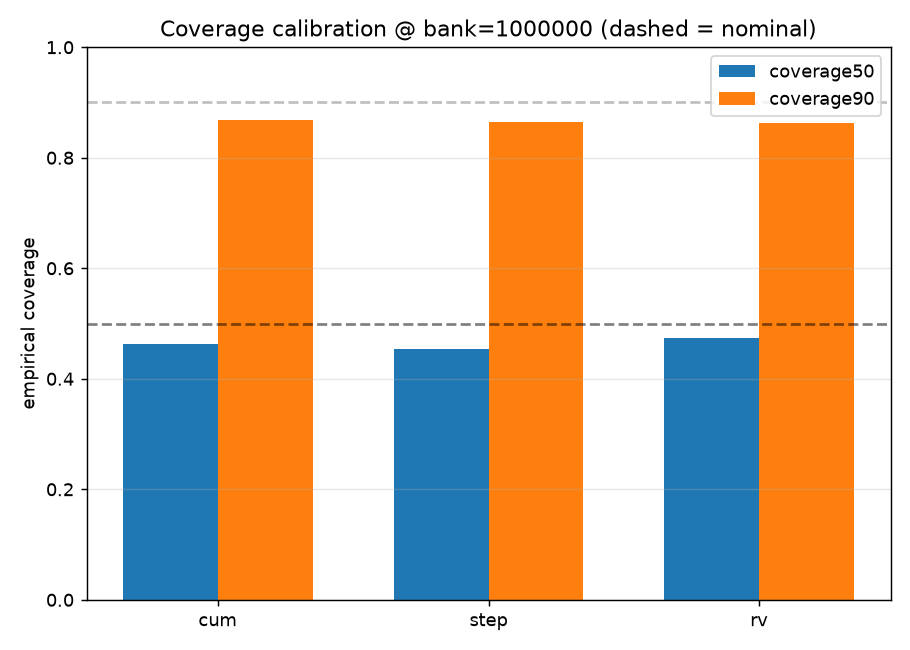
\includegraphics[width=\linewidth]{../CSDI/path_shadowing/plots/pdf_coverage_calibration.png}
\caption{CSDI --- Coverage calibration at the 1M bank; dashed lines = 0.50 / 0.90 nominal targets.}
\end{figure}
\begin{figure}[H]
\centering

\includegraphics[width=\linewidth]{../TimeDiT/baseline_no_preproc/path_shadowing/plots/pdf_crps_vs_banksize.png}
\caption{TimeDiT (raw) --- CRPS vs bank size (log $x$); solid = generator, dashed = size-matched Heston oracle, shaded = 95\% bootstrap band.}
\end{figure}
\begin{figure}[H]
\centering

\includegraphics[width=\linewidth]{../TimeDiT/baseline_no_preproc/path_shadowing/plots/pdf_coverage_calibration.png}
\caption{TimeDiT (raw) --- Coverage calibration at the 1M bank; dashed lines = 0.50 / 0.90 nominal targets.}
\end{figure}
\begin{figure}[H]
\centering

\includegraphics[width=\linewidth]{../LS4/path_shadowing/plots/pdf_crps_vs_banksize.png}
\caption{LS4 --- CRPS vs bank size (log $x$); solid = generator, dashed = size-matched Heston oracle, shaded = 95\% bootstrap band.}
\end{figure}
\begin{figure}[H]
\centering

\includegraphics[width=\linewidth]{../LS4/path_shadowing/plots/pdf_coverage_calibration.png}
\caption{LS4 --- Coverage calibration at the 1M bank; dashed lines = 0.50 / 0.90 nominal targets.}
\end{figure}
\begin{figure}[H]
\centering

\includegraphics[width=\linewidth]{../LS4/path_shadowing/plots/crps_per_step.png}
\caption{LS4 --- CRPS per horizon step.}
\end{figure}
\begin{figure}[H]
\centering

\includegraphics[width=\linewidth]{../SBTS/path_shadowing/plots/pdf_crps_vs_banksize.png}
\caption{SBTS --- CRPS vs bank size (log $x$); solid = generator, dashed = size-matched Heston oracle, shaded = 95\% bootstrap band.}
\end{figure}
\begin{figure}[H]
\centering

\includegraphics[width=\linewidth]{../SBTS/path_shadowing/plots/pdf_coverage_calibration.png}
\caption{SBTS --- Coverage calibration at the 1M bank; dashed lines = 0.50 / 0.90 nominal targets.}
\end{figure}
\subsection{Training and scoring diagnostics}
\begin{figure}[H]
\centering

\includegraphics[width=0.48\linewidth]{../CSDI/losses/loss_convergence.png}
\caption{CSDI --- training loss convergence.}
\end{figure}
\begin{figure}[H]
\centering

\includegraphics[width=0.48\linewidth]{../CSDI/plots/disc_classifier_loss.png}
\caption{CSDI --- discriminative-score classifier loss (A18).}
\end{figure}
\begin{figure}[H]
\centering

\includegraphics[width=0.48\linewidth]{../CSDI/plots/pred_score_loss.png}
\caption{CSDI --- predictive-score loss (A19).}
\end{figure}
\begin{figure}[H]
\centering

\includegraphics[width=0.48\linewidth]{../TimeDiT/losses/loss_convergence.png}
\caption{TimeDiT --- training loss convergence.}
\end{figure}
\begin{figure}[H]
\centering

\includegraphics[width=0.48\linewidth]{../TimeDiT/plots/disc_classifier_loss.png}
\caption{TimeDiT --- discriminative-score classifier loss (A18).}
\end{figure}
\begin{figure}[H]
\centering

\includegraphics[width=0.48\linewidth]{../TimeDiT/plots/pred_score_loss.png}
\caption{TimeDiT --- predictive-score loss (A19).}
\end{figure}
\begin{figure}[H]
\centering

\includegraphics[width=0.48\linewidth]{../LS4/losses/loss_convergence.png}
\caption{LS4 --- training loss convergence.}
\end{figure}
\begin{figure}[H]
\centering

\includegraphics[width=0.48\linewidth]{../LS4/plots/disc_classifier_loss.png}
\caption{LS4 --- discriminative-score classifier loss (A18).}
\end{figure}
\begin{figure}[H]
\centering

\includegraphics[width=0.48\linewidth]{../LS4/plots/pred_score_loss.png}
\caption{LS4 --- predictive-score loss (A19).}
\end{figure}
\begin{figure}[H]
\centering

\includegraphics[width=0.48\linewidth]{../SBTS/plots/disc_classifier_loss.png}
\caption{SBTS --- discriminative-score classifier loss (A18).}
\end{figure}
\begin{figure}[H]
\centering

\includegraphics[width=0.48\linewidth]{../SBTS/plots/pred_score_loss.png}
\caption{SBTS --- predictive-score loss (A19).}
\end{figure}
\subsection{Embedding visualisations (PCA / t-SNE)}
\begin{figure}[H]
\centering

\includegraphics[width=0.48\linewidth]{../CSDI/plots/seed_0_pca.png}
\caption{CSDI (log-ret) --- PCA, seed 0.}
\end{figure}
\begin{figure}[H]
\centering

\includegraphics[width=0.48\linewidth]{../CSDI/plots/seed_0_tsne.png}
\caption{CSDI (log-ret) --- t-SNE, seed 0.}
\end{figure}
\begin{figure}[H]
\centering

\includegraphics[width=0.48\linewidth]{../CSDI/plots/seed_1_pca.png}
\caption{CSDI (log-ret) --- PCA, seed 1.}
\end{figure}
\begin{figure}[H]
\centering

\includegraphics[width=0.48\linewidth]{../CSDI/plots/seed_1_tsne.png}
\caption{CSDI (log-ret) --- t-SNE, seed 1.}
\end{figure}
\begin{figure}[H]
\centering

\includegraphics[width=0.48\linewidth]{../CSDI/plots/seed_2_pca.png}
\caption{CSDI (log-ret) --- PCA, seed 2.}
\end{figure}
\begin{figure}[H]
\centering

\includegraphics[width=0.48\linewidth]{../CSDI/plots/seed_2_tsne.png}
\caption{CSDI (log-ret) --- t-SNE, seed 2.}
\end{figure}
\begin{figure}[H]
\centering

\includegraphics[width=0.48\linewidth]{../CSDI/plots/seed_3_pca.png}
\caption{CSDI (log-ret) --- PCA, seed 3.}
\end{figure}
\begin{figure}[H]
\centering

\includegraphics[width=0.48\linewidth]{../CSDI/plots/seed_3_tsne.png}
\caption{CSDI (log-ret) --- t-SNE, seed 3.}
\end{figure}
\begin{figure}[H]
\centering

\includegraphics[width=0.48\linewidth]{../CSDI/plots/seed_4_pca.png}
\caption{CSDI (log-ret) --- PCA, seed 4.}
\end{figure}
\begin{figure}[H]
\centering

\includegraphics[width=0.48\linewidth]{../CSDI/plots/seed_4_tsne.png}
\caption{CSDI (log-ret) --- t-SNE, seed 4.}
\end{figure}
\begin{figure}[H]
\centering

\includegraphics[width=0.48\linewidth]{../CSDI/baseline_no_preproc/plots/seed_0_pca.png}
\caption{CSDI (raw) --- PCA, seed 0.}
\end{figure}
\begin{figure}[H]
\centering

\includegraphics[width=0.48\linewidth]{../CSDI/baseline_no_preproc/plots/seed_0_tsne.png}
\caption{CSDI (raw) --- t-SNE, seed 0.}
\end{figure}
\begin{figure}[H]
\centering

\includegraphics[width=0.48\linewidth]{../TimeDiT/plots/seed_0_pca.png}
\caption{TimeDiT (log-ret) --- PCA, seed 0.}
\end{figure}
\begin{figure}[H]
\centering

\includegraphics[width=0.48\linewidth]{../TimeDiT/plots/seed_0_tsne.png}
\caption{TimeDiT (log-ret) --- t-SNE, seed 0.}
\end{figure}
\begin{figure}[H]
\centering

\includegraphics[width=0.48\linewidth]{../TimeDiT/plots/seed_1_pca.png}
\caption{TimeDiT (log-ret) --- PCA, seed 1.}
\end{figure}
\begin{figure}[H]
\centering

\includegraphics[width=0.48\linewidth]{../TimeDiT/plots/seed_1_tsne.png}
\caption{TimeDiT (log-ret) --- t-SNE, seed 1.}
\end{figure}
\begin{figure}[H]
\centering

\includegraphics[width=0.48\linewidth]{../TimeDiT/plots/seed_2_pca.png}
\caption{TimeDiT (log-ret) --- PCA, seed 2.}
\end{figure}
\begin{figure}[H]
\centering

\includegraphics[width=0.48\linewidth]{../TimeDiT/plots/seed_2_tsne.png}
\caption{TimeDiT (log-ret) --- t-SNE, seed 2.}
\end{figure}
\begin{figure}[H]
\centering

\includegraphics[width=0.48\linewidth]{../TimeDiT/plots/seed_3_pca.png}
\caption{TimeDiT (log-ret) --- PCA, seed 3.}
\end{figure}
\begin{figure}[H]
\centering

\includegraphics[width=0.48\linewidth]{../TimeDiT/plots/seed_3_tsne.png}
\caption{TimeDiT (log-ret) --- t-SNE, seed 3.}
\end{figure}
\begin{figure}[H]
\centering

\includegraphics[width=0.48\linewidth]{../TimeDiT/plots/seed_4_pca.png}
\caption{TimeDiT (log-ret) --- PCA, seed 4.}
\end{figure}
\begin{figure}[H]
\centering

\includegraphics[width=0.48\linewidth]{../TimeDiT/plots/seed_4_tsne.png}
\caption{TimeDiT (log-ret) --- t-SNE, seed 4.}
\end{figure}
\begin{figure}[H]
\centering

\includegraphics[width=0.48\linewidth]{../TimeDiT/baseline_no_preproc/plots/seed_0_pca.png}
\caption{TimeDiT (raw) --- PCA, seed 0.}
\end{figure}
\begin{figure}[H]
\centering

\includegraphics[width=0.48\linewidth]{../TimeDiT/baseline_no_preproc/plots/seed_0_tsne.png}
\caption{TimeDiT (raw) --- t-SNE, seed 0.}
\end{figure}
\begin{figure}[H]
\centering

\includegraphics[width=0.48\linewidth]{../LS4/plots/seed_0_pca.png}
\caption{LS4 (log-ret) --- PCA, seed 0.}
\end{figure}
\begin{figure}[H]
\centering

\includegraphics[width=0.48\linewidth]{../LS4/plots/seed_0_tsne.png}
\caption{LS4 (log-ret) --- t-SNE, seed 0.}
\end{figure}
\begin{figure}[H]
\centering

\includegraphics[width=0.48\linewidth]{../LS4/plots/seed_1_pca.png}
\caption{LS4 (log-ret) --- PCA, seed 1.}
\end{figure}
\begin{figure}[H]
\centering

\includegraphics[width=0.48\linewidth]{../LS4/plots/seed_1_tsne.png}
\caption{LS4 (log-ret) --- t-SNE, seed 1.}
\end{figure}
\begin{figure}[H]
\centering

\includegraphics[width=0.48\linewidth]{../LS4/plots/seed_2_pca.png}
\caption{LS4 (log-ret) --- PCA, seed 2.}
\end{figure}
\begin{figure}[H]
\centering

\includegraphics[width=0.48\linewidth]{../LS4/plots/seed_2_tsne.png}
\caption{LS4 (log-ret) --- t-SNE, seed 2.}
\end{figure}
\begin{figure}[H]
\centering

\includegraphics[width=0.48\linewidth]{../LS4/plots/seed_3_pca.png}
\caption{LS4 (log-ret) --- PCA, seed 3.}
\end{figure}
\begin{figure}[H]
\centering

\includegraphics[width=0.48\linewidth]{../LS4/plots/seed_3_tsne.png}
\caption{LS4 (log-ret) --- t-SNE, seed 3.}
\end{figure}
\begin{figure}[H]
\centering

\includegraphics[width=0.48\linewidth]{../LS4/plots/seed_4_pca.png}
\caption{LS4 (log-ret) --- PCA, seed 4.}
\end{figure}
\begin{figure}[H]
\centering

\includegraphics[width=0.48\linewidth]{../LS4/plots/seed_4_tsne.png}
\caption{LS4 (log-ret) --- t-SNE, seed 4.}
\end{figure}
\begin{figure}[H]
\centering

\includegraphics[width=0.48\linewidth]{../LS4/baseline_no_preproc/plots/seed_0_pca.png}
\caption{LS4 (raw) --- PCA, seed 0.}
\end{figure}
\begin{figure}[H]
\centering

\includegraphics[width=0.48\linewidth]{../LS4/baseline_no_preproc/plots/seed_0_tsne.png}
\caption{LS4 (raw) --- t-SNE, seed 0.}
\end{figure}
\begin{figure}[H]
\centering

\includegraphics[width=0.48\linewidth]{../SBTS/plots/seed_0_pca.png}
\caption{SBTS (log-ret) --- PCA, seed 0.}
\end{figure}
\begin{figure}[H]
\centering

\includegraphics[width=0.48\linewidth]{../SBTS/plots/seed_0_tsne.png}
\caption{SBTS (log-ret) --- t-SNE, seed 0.}
\end{figure}
\begin{figure}[H]
\centering

\includegraphics[width=0.48\linewidth]{../SBTS/plots/seed_1_pca.png}
\caption{SBTS (log-ret) --- PCA, seed 1.}
\end{figure}
\begin{figure}[H]
\centering

\includegraphics[width=0.48\linewidth]{../SBTS/plots/seed_1_tsne.png}
\caption{SBTS (log-ret) --- t-SNE, seed 1.}
\end{figure}
\begin{figure}[H]
\centering

\includegraphics[width=0.48\linewidth]{../SBTS/plots/seed_2_pca.png}
\caption{SBTS (log-ret) --- PCA, seed 2.}
\end{figure}
\begin{figure}[H]
\centering

\includegraphics[width=0.48\linewidth]{../SBTS/plots/seed_2_tsne.png}
\caption{SBTS (log-ret) --- t-SNE, seed 2.}
\end{figure}
\begin{figure}[H]
\centering

\includegraphics[width=0.48\linewidth]{../SBTS/plots/seed_3_pca.png}
\caption{SBTS (log-ret) --- PCA, seed 3.}
\end{figure}
\begin{figure}[H]
\centering

\includegraphics[width=0.48\linewidth]{../SBTS/plots/seed_3_tsne.png}
\caption{SBTS (log-ret) --- t-SNE, seed 3.}
\end{figure}
\begin{figure}[H]
\centering

\includegraphics[width=0.48\linewidth]{../SBTS/plots/seed_4_pca.png}
\caption{SBTS (log-ret) --- PCA, seed 4.}
\end{figure}
\begin{figure}[H]
\centering

\includegraphics[width=0.48\linewidth]{../SBTS/plots/seed_4_tsne.png}
\caption{SBTS (log-ret) --- t-SNE, seed 4.}
\end{figure}
\begin{figure}[H]
\centering

\includegraphics[width=0.48\linewidth]{../SBTS/baseline_no_preproc/plots/seed_0_pca.png}
\caption{SBTS (raw) --- PCA, seed 0.}
\end{figure}
\begin{figure}[H]
\centering

\includegraphics[width=0.48\linewidth]{../SBTS/baseline_no_preproc/plots/seed_0_tsne.png}
\caption{SBTS (raw) --- t-SNE, seed 0.}
\end{figure}
\end{document}
